
\documentclass{article}

\usepackage{lipsum}
\usepackage[margin=1in,includefoot]{geometry}
\usepackage{graphicx}
\usepackage{float}
\usepackage[hidelinks]{hyperref}
\usepackage{amsmath}
\usepackage{amssymb}
\usepackage{color}


\usepackage[usenames,dvipsnames]{xcolor}
\usepackage{listings}







% Header and Footer Stuff
\usepackage{fancyhdr}
\pagestyle{fancy}
\fancyhead{}
\fancyfoot{}
\fancyfoot[R]{\thepage}
\renewcommand{\headrulewidth}{0pt}
\renewcommand{\footrulewidth}{0pt}


\definecolor{dkgreen}{rgb}{0,0.6,0}
\definecolor{gray}{rgb}{0.5,0.5,0.5}
\definecolor{mauve}{rgb}{0.58,0,0.82}

\lstset{
  language=VHDL,
  aboveskip=3mm,
  belowskip=3mm,
  showstringspaces=false,
  columns=flexible,
  basicstyle={\small\ttfamily},
  numbers=none,
  numberstyle=\tiny\color{gray},
  keywordstyle=\color{blue},
  commentstyle=\color{dkgreen},
  stringstyle=\color{mauve},
  breaklines=true,
  breakatwhitespace=true,
  tabsize=3
}












\begin{document}

\begin{titlepage}
	\begin{center}
	\begin{align*}
	
\includegraphics[height=1.75in]{logo.png}
	\end{align*}


	
	\line(1,0){300}\\
	[0.25in]
	\huge{\bfseries Datapath Design}\\
	[2mm]
	\line(1,0){200}\\
	[1.5cm]
	\textsc{\LARGE Laboratory 1}\\
	[0.75cm]
	\textsc{\Large CS2022 Computer Architecture}\\
	[7cm]	
	\end{center}
	
	
	
	\begin{flushright}
	\textsc{\large Alexandru Sulea\\
	D Stream\\
	\#12315152\\
	19 Februrary 2015\\}
	\end{flushright}
	
	
	
	

\end{titlepage}
%Table of Contents Stuff%
\tableofcontents
%\listoffigures
%\addcontentsline{toc}{section}{List of Figures}
\listoftables
\addcontentsline{toc}{section}{List of Tables}


\thispagestyle{empty}
\cleardoublepage
\pagenumbering{arabic}
\setcounter{page}{1}

\pagebreak
\section{CODE}

\subsection{REGISTER FILE}\label{sec:intro}

\begin{lstlisting}
library IEEE;
use IEEE.STD_LOGIC_1164.ALL;
use IEEE.STD_LOGIC_ARITH.ALL;
use IEEE.STD_LOGIC_UNSIGNED.ALL;


entity register_file is
    Port ( src_S0 : in  STD_LOGIC;
           src_S1 : in  STD_LOGIC;
           src_S2 : in  STD_LOGIC;
           des_A0 : in  STD_LOGIC;
           des_A1 : in  STD_LOGIC;
           des_A2 : in  STD_LOGIC;
           Clk : in  STD_LOGIC;
           data_src : in  STD_LOGIC;
           data : in  STD_LOGIC_VECTOR(15 downto 0);
           reg0 : out  STD_LOGIC_VECTOR(15 downto 0);
           reg1 : out  STD_LOGIC_VECTOR(15 downto 0);
           reg2 : out  STD_LOGIC_VECTOR(15 downto 0);
           reg3 : out  STD_LOGIC_VECTOR(15 downto 0);
           reg4 : out  STD_LOGIC_VECTOR(15 downto 0);
           reg5 : out  STD_LOGIC_VECTOR(15 downto 0);
           reg6 : out  STD_LOGIC_VECTOR(15 downto 0);
           reg7 : out  STD_LOGIC_VECTOR(15 downto 0));
end register_file;

architecture Behavioral of register_file is

	Component decoder_3to8
	Port ( A0 : in  STD_LOGIC;
          A1 : in  STD_LOGIC;
			 A2 : in  STD_LOGIC;
          Q0 : out  STD_LOGIC;
          Q1 : out  STD_LOGIC;
          Q2 : out  STD_LOGIC;
          Q3 : out  STD_LOGIC;
          Q4 : out  STD_LOGIC;
          Q5 : out  STD_LOGIC;
          Q6 : out  STD_LOGIC;
          Q7 : out  STD_LOGIC);
	End Component;

	Component mux3_16bit
	Port ( s : in  STD_LOGIC;
          In0 : in  STD_LOGIC_VECTOR(15 downto 0);
          In1 : in  STD_LOGIC_VECTOR(15 downto 0);
          Z : out  STD_LOGIC_VECTOR(15 downto 0));
	End Component;
	
	Component reg8
	Port ( load : in  STD_LOGIC;
          Clk : in  STD_LOGIC;
          D : in  STD_LOGIC_VECTOR(15 downto 0);
          Q : out  STD_LOGIC_VECTOR(15 downto 0));
	End Component;
	
	Component mux8_16bit
	Port ( S0 : in  STD_LOGIC;
           S1 : in  STD_LOGIC;
           S2 : in  STD_LOGIC;
           In0 : in  STD_LOGIC_VECTOR(15 downto 0);
           In1 : in  STD_LOGIC_VECTOR(15 downto 0);
           In2 : in  STD_LOGIC_VECTOR(15 downto 0);
           In3 : in  STD_LOGIC_VECTOR(15 downto 0);
           In4 : in  STD_LOGIC_VECTOR(15 downto 0);
           In5 : in  STD_LOGIC_VECTOR(15 downto 0);
           In6 : in  STD_LOGIC_VECTOR(15 downto 0);
           In7 : in  STD_LOGIC_VECTOR(15 downto 0);
           Z : out  STD_LOGIC_VECTOR(15 downto 0));
	End Component;
	
	signal load_reg0, load_reg1, load_reg2, load_reg3, load_reg4,
				load_reg5, load_reg6, load_reg7 : STD_LOGIC;
	signal reg0_q, reg1_q, reg2_q, reg3_q, reg4_q, reg5_q, reg6_q,
				reg7_q, d_mux, src_reg : STD_LOGIC_VECTOR(15 downto 0);

begin
	reg_decoder_3to8 : decoder_3to8 PORT MAP(
		A0 => des_A0,
		A1 => des_A1,
		A2 => des_A2,
		Q0 => load_reg0,
		Q1 => load_reg1,
		Q2 => load_reg2,
		Q3 => load_reg3,
		Q4 => load_reg4,
		Q5 => load_reg5,
		Q6 => load_reg6,
		Q7 => load_reg7
		);
	reg_mux3_16bit : mux3_16bit PORT MAP(
		s =>	data_src, 
		In0 => data,
		In1 => src_reg,
		Z =>	d_mux
		);
	reg_mux8_16bit : mux8_16bit PORT MAP(
		S0 => src_s0,
		S1 => src_s1,
		S2 => src_s2,
		In0 => reg0_q,
		In1 => reg1_q,
		In2 => reg2_q,
		In3 => reg3_q,
		In4 => reg4_q,
		In5 => reg5_q,
		In6 => reg6_q,
		In7 => reg7_q,
		Z => src_reg
		);
		
	reg00 : reg8 PORT MAP(
		load =>	load_reg0,
		Clk =>	Clk,
		D =>	d_mux,
		Q => reg0_q);
		
	reg01 : reg8 PORT MAP(
		load =>	load_reg1,
		Clk =>	Clk,
		D =>	d_mux,
		Q => reg1_q);
	
	reg02 : reg8 PORT MAP(
		load =>	load_reg2,
		Clk =>	Clk,
		D =>	d_mux,
		Q => reg2_q);	

	reg03 : reg8 PORT MAP(
		load =>	load_reg3,
		Clk =>	Clk,
		D =>	d_mux,
		Q => reg3_q);

	reg04 : reg8 PORT MAP(
		load =>	load_reg4,
		Clk =>	Clk,
		D =>	d_mux,
		Q => reg4_q);
		
	reg05 : reg8 PORT MAP(
		load =>	load_reg5,
		Clk =>	Clk,
		D =>	d_mux,
		Q => reg5_q);
		
	reg06 : reg8 PORT MAP(
		load =>	load_reg6,
		Clk =>	Clk,
		D =>	d_mux,
		Q => reg6_q);
		
	reg07 : reg8 PORT MAP(
		load =>	load_reg7,
		Clk =>	Clk,
		D =>	d_mux,
		Q => reg7_q);

	reg0 <= reg0_q;
	reg1 <= reg1_q;
	reg2 <= reg2_q;
	reg3 <= reg3_q;
	reg4 <= reg4_q;
	reg5 <= reg5_q;
	reg6 <= reg6_q;
	reg7 <= reg7_q;

end Behavioral;
\end{lstlisting}



\begin{align*}
\centering
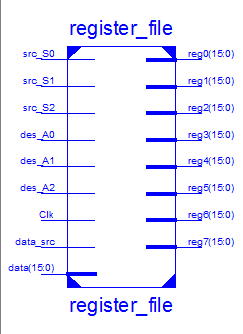
\includegraphics[height=3in]{reg.png}
\break
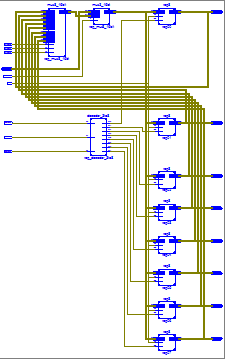
\includegraphics[height=3in]{all.png}
\end{align*}\\



\pagebreak
\subsection{REG8}\label{sec:result}

\begin{lstlisting}
library IEEE;
use IEEE.STD_LOGIC_1164.ALL;
use IEEE.STD_LOGIC_ARITH.ALL;
use IEEE.STD_LOGIC_UNSIGNED.ALL;
entity reg8 is
    Port ( load : in  STD_LOGIC;
           Clk : in  STD_LOGIC;
           D : in  STD_LOGIC_VECTOR(15 downto 0);
           Q : out  STD_LOGIC_VECTOR(15 downto 0));
end reg8;

architecture Behavioral of reg8 is

begin
process(Clk)
begin 
		if(rising_edge(Clk)) then 
			if(load ='1') then 
				Q<= D after 5ns;
			end if;
		end if;
	end process;
end Behavioral;
\end{lstlisting}

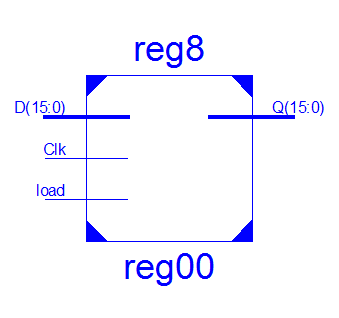
\includegraphics[width=6cm, height=8cm]{reg8.png}


\pagebreak
\subsection{DECODER}\label{sec:result}

\begin{lstlisting}
library IEEE;
use IEEE.STD_LOGIC_1164.ALL;
use IEEE.STD_LOGIC_ARITH.ALL;
use IEEE.STD_LOGIC_UNSIGNED.ALL;


entity decoder_3to8 is
    Port ( A0 : in  STD_LOGIC;
           A1 : in  STD_LOGIC;
           A2 : in  STD_LOGIC;
           Q0 : out  STD_LOGIC;
           Q1 : out  STD_LOGIC;
           Q2 : out  STD_LOGIC;
           Q3 : out  STD_LOGIC;
           Q4 : out  STD_LOGIC;
           Q5 : out  STD_LOGIC;
           Q6 : out  STD_LOGIC;
           Q7 : out  STD_LOGIC);
end decoder_3to8;

architecture Behavioral of decoder_3to8 is

begin
	Q0 <= ((	NOT A0) AND (NOT A1) AND (NOT A2)) AFTER 5ns;
	Q1 <= ((	NOT A0) AND (NOT A1) AND A2) AFTER 5ns;
	Q2 <= ((	NOT A0) AND A1 AND (NOT A2)) AFTER 5ns;
	Q3 <= ((	NOT A0) AND A1 AND A2) AFTER 5ns;
	Q4 <= (A0 AND (NOT A1) AND (NOT A2)) AFTER 5ns;
	Q5 <= (A0 AND (NOT A1) AND A2) AFTER 5ns;
	Q6 <= (A0 AND A1 AND (NOT A2)) AFTER 5ns;
	Q7 <= (A0 AND A1 AND A2) AFTER 5ns;


end Behavioral;
\end{lstlisting}

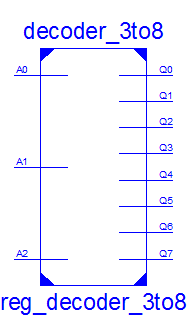
\includegraphics[width=5cm, height=7cm]{decoder.png}
\pagebreak
\subsection{MUX3}\label{sec:result}

\begin{lstlisting}

library IEEE;
use IEEE.STD_LOGIC_1164.ALL;
use IEEE.STD_LOGIC_ARITH.ALL;
use IEEE.STD_LOGIC_UNSIGNED.ALL;


entity mux3_16bit is
    Port ( s : in  STD_LOGIC;
           In0 : in  STD_LOGIC_VECTOR(15 downto 0);
           In1 : in  STD_LOGIC_VECTOR(15 downto 0);
           Z : out  STD_LOGIC_VECTOR(15 downto 0));
end mux3_16bit;

architecture Behavioral of mux3_16bit is

begin
	Z <= In0 after 5ns when s = '0' else
			In1 after 5ns when s = '1' else
			x"0000" after 5ns;

end Behavioral;
\end{lstlisting}

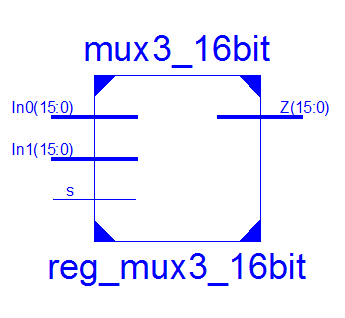
\includegraphics[width=6cm, height=8cm]{mux3.png}

\pagebreak
\subsection{MUX8}\label{sec:result}

\begin{lstlisting}

library IEEE;
use IEEE.STD_LOGIC_1164.ALL;
use IEEE.STD_LOGIC_ARITH.ALL;
use IEEE.STD_LOGIC_UNSIGNED.ALL;

entity mux8_16bit is
    Port ( S0 : in  STD_LOGIC;
           S1 : in  STD_LOGIC;
           S2 : in  STD_LOGIC;
           In0 : in  STD_LOGIC_VECTOR(15 downto 0);
           In1 : in  STD_LOGIC_VECTOR(15 downto 0);
           In2 : in  STD_LOGIC_VECTOR(15 downto 0);
           In3 : in  STD_LOGIC_VECTOR(15 downto 0);
           In4 : in  STD_LOGIC_VECTOR(15 downto 0);
           In5 : in  STD_LOGIC_VECTOR(15 downto 0);
           In6 : in  STD_LOGIC_VECTOR(15 downto 0);
           In7 : in  STD_LOGIC_VECTOR(15 downto 0);
           Z : out  STD_LOGIC_VECTOR(15 downto 0));
end mux8_16bit;

architecture Behavioral of mux8_16bit is

begin
	Z <= In0 after 5ns when S0 = '0' and S1 = '0' and S2 = '0' else 
			In1 after 5ns when S0 = '0' and S1 = '0' and S2 = '1' else 
			In2 after 5ns when S0 = '0' and S1 = '1' and S2 = '0' else 
			In3 after 5ns when S0 = '0' and S1 = '1' and S2 = '1' else
			In4 after 5ns when S0 = '1' and S1 = '0' and S2 = '0' else
			In5 after 5ns when S0 = '1' and S1 = '0' and S2 = '1' else
			In6 after 5ns when S0 = '1' and S1 = '1' and S2 = '0' else
			In7 after 5ns when S0 = '1' and S1 = '1' and S2 = '1' else
			x"0000" after 5ns;
end Behavioral;

\end{lstlisting}

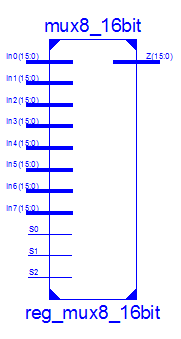
\includegraphics[width=5cm, height=7cm]{mux8.png}






\pagebreak

\section{TESTBENCHES}

\subsection{REGISTER FILE 1}\label{sec:result}

\begin{lstlisting}
LIBRARY ieee;
USE ieee.std_logic_1164.ALL;
 
-- Uncomment the following library declaration if using
-- arithmetic functions with Signed or Unsigned values
--USE ieee.numeric_std.ALL;
 
ENTITY test_register_file IS
END test_register_file;
 
ARCHITECTURE behavior OF test_register_file IS 
 
    -- Component Declaration for the Unit Under Test (UUT)
 
    COMPONENT register_file
    PORT(
         src_S0 : IN  std_logic;
         src_S1 : IN  std_logic;
         src_S2 : IN  std_logic;
         des_A0 : IN  std_logic;
         des_A1 : IN  std_logic;
         des_A2 : IN  std_logic;
         Clk : IN  std_logic;
         data_src : IN  std_logic;
         data : IN  std_logic_vector(15 downto 0);
         reg0 : OUT  std_logic_vector(15 downto 0);
         reg1 : OUT  std_logic_vector(15 downto 0);
         reg2 : OUT  std_logic_vector(15 downto 0);
         reg3 : OUT  std_logic_vector(15 downto 0);
         reg4 : OUT  std_logic_vector(15 downto 0);
         reg5 : OUT  std_logic_vector(15 downto 0);
         reg6 : OUT  std_logic_vector(15 downto 0);
         reg7 : OUT  std_logic_vector(15 downto 0)
        );
    END COMPONENT;
    

   --Inputs
   signal src_S0 : std_logic := '0';
   signal src_S1 : std_logic := '0';
   signal src_S2 : std_logic := '0';
   signal des_A0 : std_logic := '0';
   signal des_A1 : std_logic := '0';
   signal des_A2 : std_logic := '0';
   signal Clk : std_logic := '0';
   signal data_src : std_logic := '0';
   signal data : std_logic_vector(15 downto 0) := (others => '0');

 	--Outputs
   signal reg0 : std_logic_vector(15 downto 0);
   signal reg1 : std_logic_vector(15 downto 0);
   signal reg2 : std_logic_vector(15 downto 0);
   signal reg3 : std_logic_vector(15 downto 0);
   signal reg4 : std_logic_vector(15 downto 0);
   signal reg5 : std_logic_vector(15 downto 0);
   signal reg6 : std_logic_vector(15 downto 0);
   signal reg7 : std_logic_vector(15 downto 0);

   -- Clock period definitions
   constant Clk_period : time := 10 ns;
 
BEGIN
 
	-- Instantiate the Unit Under Test (UUT)
   uut: register_file PORT MAP (
          src_S0 => src_S0,
          src_S1 => src_S1,
          src_S2 => src_S2,
          des_A0 => des_A0,
          des_A1 => des_A1,
          des_A2 => des_A2,
          Clk => Clk,
          data_src => data_src,
          data => data,
          reg0 => reg0,
          reg1 => reg1,
          reg2 => reg2,
          reg3 => reg3,
          reg4 => reg4,
          reg5 => reg5,
          reg6 => reg6,
          reg7 => reg7
        );

   -- Clock process definitions
   Clk_process :process
   begin
		Clk <= '0';
		wait for Clk_period/2;
		Clk <= '1';
		wait for Clk_period/2;
   end process;
 

   -- Stimulus process
   stim_proc: process
   begin		
		wait for 10 ns;
			des_A0 <= '0';
			des_A1 <= '0';
			des_A2 <= '0';
			data <= x"FFFF";
		
		wait for 10 ns;
			des_A0 <= '0';
			des_A1 <= '0';
			des_A2 <= '1';
			data <= x"EEEE";
			
		wait for 10 ns;
			des_A0 <= '0';
			des_A1 <= '1';
			des_A2 <= '0';
			data <= x"DDDD";
		
		wait for 10 ns;
			des_A0 <= '0';
			des_A1 <= '1';
			des_A2 <= '1';
			data <= x"CCCC";
			
			wait for 10 ns;
			des_A0 <= '1';
			des_A1 <= '0';
			des_A2 <= '0';
			data <= x"BBBB";
		
		wait for 10 ns;
			des_A0 <= '1';
			des_A1 <= '0';
			des_A2 <= '1';
			data <= x"AAAA";
			
		wait for 10 ns;
			des_A0 <= '1';
			des_A1 <= '1';
			des_A2 <= '0';
			data <= x"9999";
		
		wait for 10 ns;
			des_A0 <= '1';
			des_A1 <= '1';
			des_A2 <= '1';
			data <= x"0000";
	  
    
   end process;

END;
\end{lstlisting}
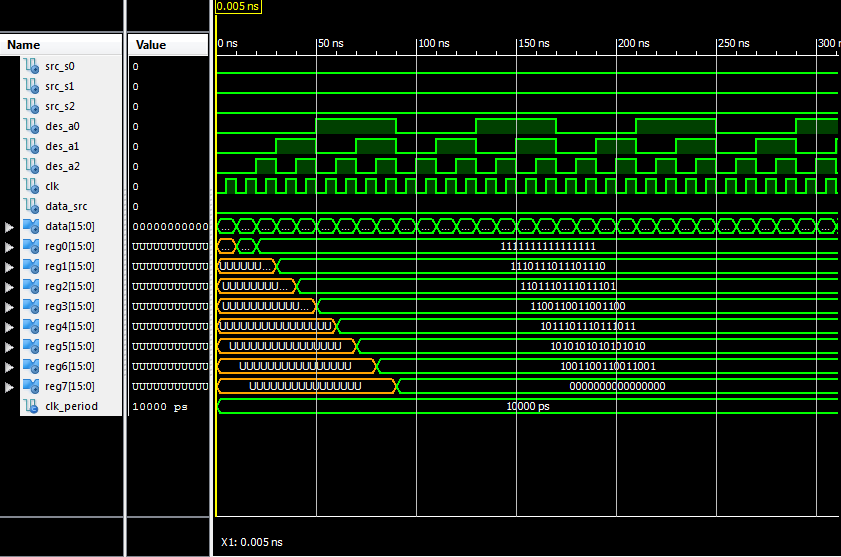
\includegraphics[width=10cm, height=5cm]{test_reg_file.png}

\pagebreak

\subsection{REGISTER FILE 2}\label{sec:result}

\begin{lstlisting}
LIBRARY ieee;
USE ieee.std_logic_1164.ALL;
 
-- Uncomment the following library declaration if using
-- arithmetic functions with Signed or Unsigned values
--USE ieee.numeric_std.ALL;
 
ENTITY test_register_file_2 IS
END test_register_file_2;
 
ARCHITECTURE behavior OF test_register_file_2 IS 
 
    -- Component Declaration for the Unit Under Test (UUT)
 
    COMPONENT register_file
    PORT(
         src_S0 : IN  std_logic;
         src_S1 : IN  std_logic;
         src_S2 : IN  std_logic;
         des_A0 : IN  std_logic;
         des_A1 : IN  std_logic;
         des_A2 : IN  std_logic;
         Clk : IN  std_logic;
         data_src : IN  std_logic;
         data : IN  std_logic_vector(15 downto 0);
         reg0 : OUT  std_logic_vector(15 downto 0);
         reg1 : OUT  std_logic_vector(15 downto 0);
         reg2 : OUT  std_logic_vector(15 downto 0);
         reg3 : OUT  std_logic_vector(15 downto 0);
         reg4 : OUT  std_logic_vector(15 downto 0);
         reg5 : OUT  std_logic_vector(15 downto 0);
         reg6 : OUT  std_logic_vector(15 downto 0);
         reg7 : OUT  std_logic_vector(15 downto 0)
        );
    END COMPONENT;
    

   --Inputs
   signal src_S0 : std_logic := '0';
   signal src_S1 : std_logic := '0';
   signal src_S2 : std_logic := '0';
   signal des_A0 : std_logic := '0';
   signal des_A1 : std_logic := '0';
   signal des_A2 : std_logic := '0';
   signal Clk : std_logic := '0';
   signal data_src : std_logic := '0';
   signal data : std_logic_vector(15 downto 0) := (others => '0');

 	--Outputs
   signal reg0 : std_logic_vector(15 downto 0);
   signal reg1 : std_logic_vector(15 downto 0);
   signal reg2 : std_logic_vector(15 downto 0);
   signal reg3 : std_logic_vector(15 downto 0);
   signal reg4 : std_logic_vector(15 downto 0);
   signal reg5 : std_logic_vector(15 downto 0);
   signal reg6 : std_logic_vector(15 downto 0);
   signal reg7 : std_logic_vector(15 downto 0);

   -- Clock period definitions
   constant Clk_period : time := 10 ns;
 
BEGIN
 
	-- Instantiate the Unit Under Test (UUT)
   uut: register_file PORT MAP (
          src_S0 => src_S0,
          src_S1 => src_S1,
          src_S2 => src_S2,
          des_A0 => des_A0,
          des_A1 => des_A1,
          des_A2 => des_A2,
          Clk => Clk,
          data_src => data_src,
          data => data,
          reg0 => reg0,
          reg1 => reg1,
          reg2 => reg2,
          reg3 => reg3,
          reg4 => reg4,
          reg5 => reg5,
          reg6 => reg6,
          reg7 => reg7
        );

   -- Clock process definitions
   Clk_process :process
   begin
		Clk <= '0';
		wait for Clk_period/2;
		Clk <= '1';
		wait for Clk_period/2;
   end process;
 

   -- Stimulus process
   stim_proc: process
   begin		
      

      wait for 10ns;
			data <= x"FFFF";
			des_A0 <= '0';
			des_A1 <= '0';
			des_A2 <= '0';
		
			src_S0 <= '0';
			src_S0 <= '0';
			src_S0 <= '0';
			
		wait for 20ns;
			data <= x"EEEE";
			des_A0 <= '0';
			des_A1 <= '0';
			des_A2 <= '1';
		
			src_S0 <= '0';
			src_S0 <= '0';
			src_S0 <= '1';
			
		wait for 30ns;
			data <= x"DDDD";
			des_A0 <= '0';
			des_A1 <= '1';
			des_A2 <= '0';
		
			src_S0 <= '0';
			src_S0 <= '1';
			src_S0 <= '0';
			
		wait for 40ns;
			data <= x"CCCC";
			des_A0 <= '0';
			des_A1 <= '1';
			des_A2 <= '1';
		
			src_S0 <= '0';
			src_S0 <= '1';
			src_S0 <= '1';
			
			
		 wait for 50ns;
			data <= x"BBBB";
			des_A0 <= '1';
			des_A1 <= '0';
			des_A2 <= '0';
		
			src_S0 <= '1';
			src_S0 <= '0';
			src_S0 <= '0';
			
		wait for 60ns;
			data <= x"AAAA";
			des_A0 <= '1';
			des_A1 <= '0';
			des_A2 <= '1';
		
			src_S0 <= '1';
			src_S0 <= '0';
			src_S0 <= '1';
			
		wait for 70ns;
			data <= x"9999";
			des_A0 <= '1';
			des_A1 <= '1';
			des_A2 <= '0';
		
			src_S0 <= '1';
			src_S0 <= '1';
			src_S0 <= '0';
			
		wait for 80ns;
			data <= x"0000";
			des_A0 <= '1';
			des_A1 <= '1';
			des_A2 <= '1';
		
			src_S0 <= '1';
			src_S0 <= '1';
			src_S0 <= '1';
			
   end process;

END;
\end{lstlisting}

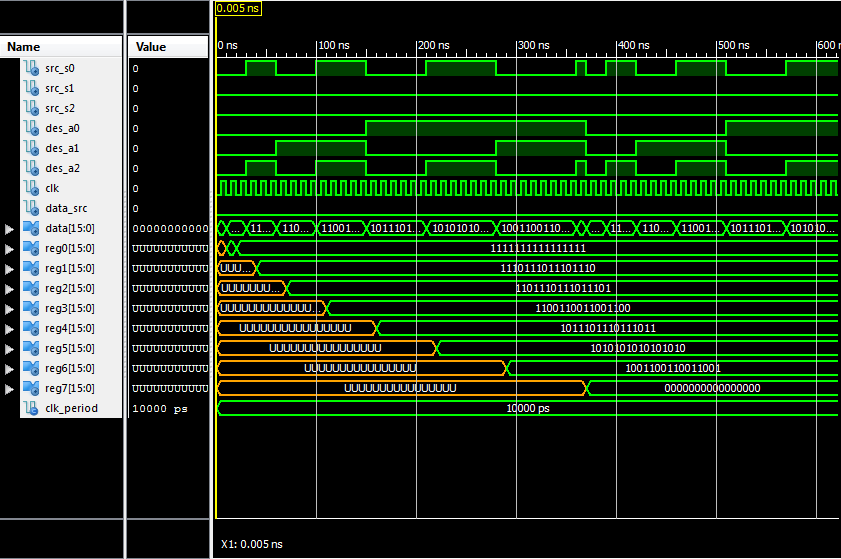
\includegraphics[width=16cm, height=8cm]{test_reg_file_2.png}
\pagebreak

\subsection{REG8}\label{sec:result}

\begin{lstlisting}
LIBRARY ieee;
USE ieee.std_logic_1164.ALL;
 

 
ENTITY test_reg8 IS
END test_reg8;
 
ARCHITECTURE behavior OF test_reg8 IS 
 
    -- Component Declaration for the Unit Under Test (UUT)
 
    COMPONENT reg8
    PORT(
         load : IN  std_logic;
         Clk : IN  std_logic;
         D : IN  std_logic_vector(15 downto 0);
         Q : OUT  std_logic_vector(15 downto 0)
        );
    END COMPONENT;
    

   --Inputs
   signal load : std_logic := '0';
   signal Clk : std_logic := '0';
   signal D : std_logic_vector(15 downto 0) := (others => '0');

 	--Outputs
   signal Q : std_logic_vector(15 downto 0);

   -- Clock period definitions
   constant Clk_period : time := 10 ns;
 
BEGIN
 
	-- Instantiate the Unit Under Test (UUT)
   uut: reg8 PORT MAP (
          load => load,
          Clk => Clk,
          D => D,
          Q => Q
        );

   -- Clock process definitions
   Clk_process :process
   begin
		Clk <= '0';
		wait for Clk_period/2;
		Clk <= '1';
		wait for Clk_period/2;
   end process;
 

   -- Stimulus process
   stim_proc: process
   begin		
	wait for 10ns;
	D <= x"FFFF";
	load <= '1';
	
	wait for 10ns;
	load <= '0';
	
	wait for 10ns;
	D<= x"AAAA";
	load <= '1';
	
      
   wait for 10ns;
	load <= '0';
	
   end process;
END;
\end{lstlisting}
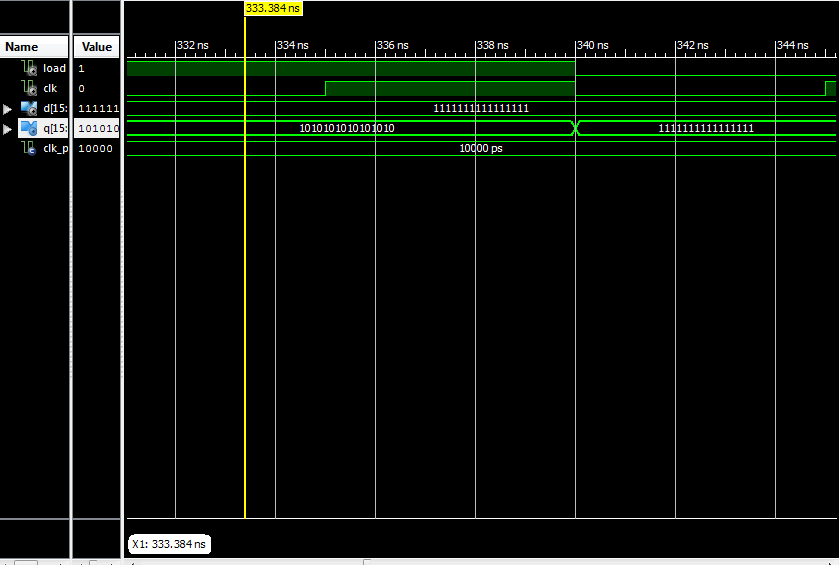
\includegraphics[width=16cm, height=8cm]{test_reg8.png}
\pagebreak
\subsection{DECODER}\label{sec:result}

\begin{lstlisting}
LIBRARY ieee;
USE ieee.std_logic_1164.ALL;
 
-- Uncomment the following library declaration if using
-- arithmetic functions with Signed or Unsigned values
--USE ieee.numeric_std.ALL;
 
ENTITY test_decoder_3to8 IS
END test_decoder_3to8;
 
ARCHITECTURE behavior OF test_decoder_3to8 IS 
 
    -- Component Declaration for the Unit Under Test (UUT)
 
    COMPONENT decoder_3to8
    PORT(
         A0 : IN  std_logic;
         A1 : IN  std_logic;
         A2 : IN  std_logic;
         Q0 : OUT  std_logic;
         Q1 : OUT  std_logic;
         Q2 : OUT  std_logic;
         Q3 : OUT  std_logic;
         Q4 : OUT  std_logic;
         Q5 : OUT  std_logic;
         Q6 : OUT  std_logic;
         Q7 : OUT  std_logic
        );
    END COMPONENT;
    

   --Inputs
   signal A0 : std_logic := '0';
   signal A1 : std_logic := '0';
   signal A2 : std_logic := '0';

 	--Outputs
   signal Q0 : std_logic;
   signal Q1 : std_logic;
   signal Q2 : std_logic;
   signal Q3 : std_logic;
   signal Q4 : std_logic;
   signal Q5 : std_logic;
   signal Q6 : std_logic;
   signal Q7 : std_logic;
   
BEGIN
 
	-- Instantiate the Unit Under Test (UUT)
   uut: decoder_3to8 PORT MAP (
          A0 => A0,
          A1 => A1,
          A2 => A2,
          Q0 => Q0,
          Q1 => Q1,
          Q2 => Q2,
          Q3 => Q3,
          Q4 => Q4,
          Q5 => Q5,
          Q6 => Q6,
          Q7 => Q7
        );

 
   -- Stimulus process
   stim_proc: process
   begin		
     wait for 10ns;
	  A0 <= '0';
	  A1 <= '0';
	  A2 <= '0';
	  
	  wait for 10ns;
	  A0 <= '0';
	  A1 <= '0';
	  A2 <= '1';
	  
	  wait for 10ns;
	  A0 <= '0';
	  A1 <= '1';
	  A2 <= '0';
	  
	  wait for 10ns;
	  A0 <= '0';
	  A1 <= '1';
	  A2 <= '1';

	  wait for 10ns;
	  A0 <= '1';
	  A1 <= '0';
	  A2 <= '0';
	  
	  wait for 10ns;
	  A0 <= '1';
	  A1 <= '0';
	  A2 <= '1';
	  
	  wait for 10ns;
	  A0 <= '1';
	  A1 <= '1';
	  A2 <= '0';
	  
	  wait for 10ns;
	  A0 <= '1';
	  A1 <= '1';
	  A2 <= '1';

   end process;

END;
\end{lstlisting}
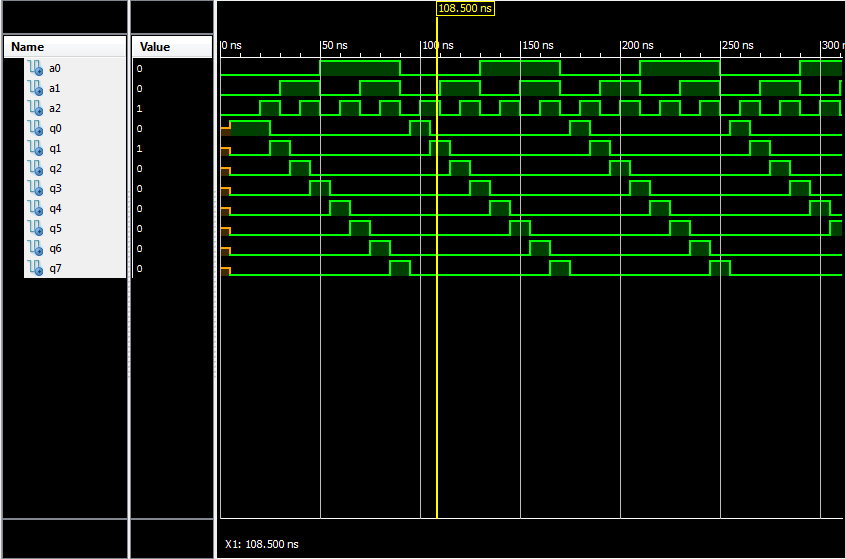
\includegraphics[width=16cm, height=8cm]{test_decoder.png}

\pagebreak

\subsection{MUX3}\label{sec:result}

\begin{lstlisting}
LIBRARY ieee;
USE ieee.std_logic_1164.ALL;
 

 
ENTITY test_mux3_16bit IS
END test_mux3_16bit;
 
ARCHITECTURE behavior OF test_mux3_16bit IS 
 
  
 
    COMPONENT mux3_16bit
    PORT(
         s : IN  std_logic;
         In0 : IN  std_logic_vector(15 downto 0);
         In1 : IN  std_logic_vector(15 downto 0);
         Z : OUT  std_logic_vector(15 downto 0)
        );
    END COMPONENT;
    

   --Inputs for the in0 and in1
   signal s : std_logic := '0';
   signal In0 : std_logic_vector(15 downto 0) := (others => '0');
   signal In1 : std_logic_vector(15 downto 0) := (others => '0');

 	--Outputs
   signal Z : std_logic_vector(15 downto 0);
   -- No clocks detected in port list. Replace <clock> below with 
   -- appropriate port name 
 
  
BEGIN
 
	-- Instantiate the Unit Under Test (UUT)
   uut: mux3_16bit PORT MAP (
          s => s,
          In0 => In0,
          In1 => In1,
          Z => Z
        );

   -- Signasl tested are here below
   stim_proc: process
   begin		
		wait for 10ns;
		In0<= x"FFFF";
		In1<= X"AAAA";
		
		wait for 10ns;
		s <= '1';
		
		wait for 10ns;
		s <= '0';
		
		wait for 10ns;
		s <= '0';
  
      wait;
   end process;

END;
\end{lstlisting}
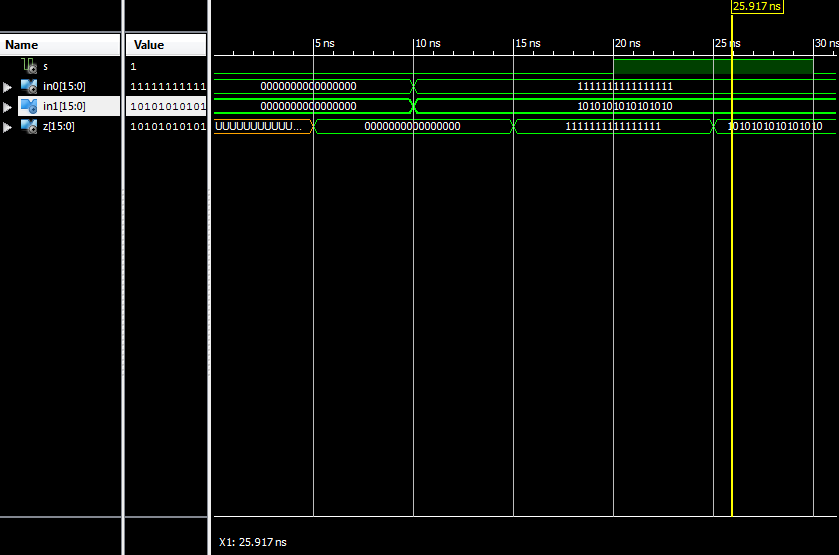
\includegraphics[width=16cm, height=8cm]{test_mux3.png}
\pagebreak

\subsection{MUX8}\label{sec:result}

\begin{lstlisting}
LIBRARY ieee;
USE ieee.std_logic_1164.ALL;
 
-- Uncomment the following library declaration if using
-- arithmetic functions with Signed or Unsigned values
--USE ieee.numeric_std.ALL;
 
ENTITY test_mux8_16bit IS
END test_mux8_16bit;
 
ARCHITECTURE behavior OF test_mux8_16bit IS 
 
    -- Component Declaration for the Unit Under Test (UUT)
 
    COMPONENT mux8_16bit
    PORT(
         S0 : IN  std_logic;
         S1 : IN  std_logic;
         S2 : IN  std_logic;
         In0 : IN  std_logic_vector(15 downto 0);
         In1 : IN  std_logic_vector(15 downto 0);
         In2 : IN  std_logic_vector(15 downto 0);
         In3 : IN  std_logic_vector(15 downto 0);
         In4 : IN  std_logic_vector(15 downto 0);
         In5 : IN  std_logic_vector(15 downto 0);
         In6 : IN  std_logic_vector(15 downto 0);
         In7 : IN  std_logic_vector(15 downto 0);
         Z : OUT  std_logic_vector(15 downto 0)
        );
    END COMPONENT;
    

   --Inputs
   signal S0 : std_logic := '0';
   signal S1 : std_logic := '0';
   signal S2 : std_logic := '0';
   signal In0 : std_logic_vector(15 downto 0) := (others => '0');
   signal In1 : std_logic_vector(15 downto 0) := (others => '0');
   signal In2 : std_logic_vector(15 downto 0) := (others => '0');
   signal In3 : std_logic_vector(15 downto 0) := (others => '0');
   signal In4 : std_logic_vector(15 downto 0) := (others => '0');
   signal In5 : std_logic_vector(15 downto 0) := (others => '0');
   signal In6 : std_logic_vector(15 downto 0) := (others => '0');
   signal In7 : std_logic_vector(15 downto 0) := (others => '0');

 	--Outputs
   signal Z : std_logic_vector(15 downto 0);
  
BEGIN
 
	-- Instantiate the Unit Under Test (UUT)
   uut: mux8_16bit PORT MAP (
          S0 => S0,
          S1 => S1,
          S2 => S2,
          In0 => In0,
          In1 => In1,
          In2 => In2,
          In3 => In3,
          In4 => In4,
          In5 => In5,
          In6 => In6,
          In7 => In7,
          Z => Z
        );

 
   -- Stimulus process
   stim_proc: process
   begin		
	
		In0 <= x"FFFF";
		In0 <= x"EEEE";
		In0 <= x"DDDD";
		In0 <= x"CCCC";
		In0 <= x"BBBB";
		In0 <= x"AAAA";
		In0 <= x"9999";
		In0 <= x"0000";
     
		wait for 10ns;
		S0 <= '0';
		S1 <= '0';
		S2 <= '0';
		
		wait for 10ns;
		S0 <= '0';
		S1 <= '0';
		S2 <= '1';
		
		wait for 10ns;
		S0 <= '0';
		S1 <= '1';
		S2 <= '0';
		
		wait for 10ns;
		S0 <= '0';
		S1 <= '1';
		S2 <= '1';
		
		wait for 10ns;
		S0 <= '1';
		S1 <= '0';
		S2 <= '0';
		
		wait for 10ns;
		S0 <= '1';
		S1 <= '0';
		S2 <= '1';
		
		wait for 10ns;
		S0 <= '1';
		S1 <= '1';
		S2 <= '0';
		
		wait for 10ns;
		S0 <= '1';
		S1 <= '1';
		S2 <= '1';
   end process;

END;
\end{lstlisting}
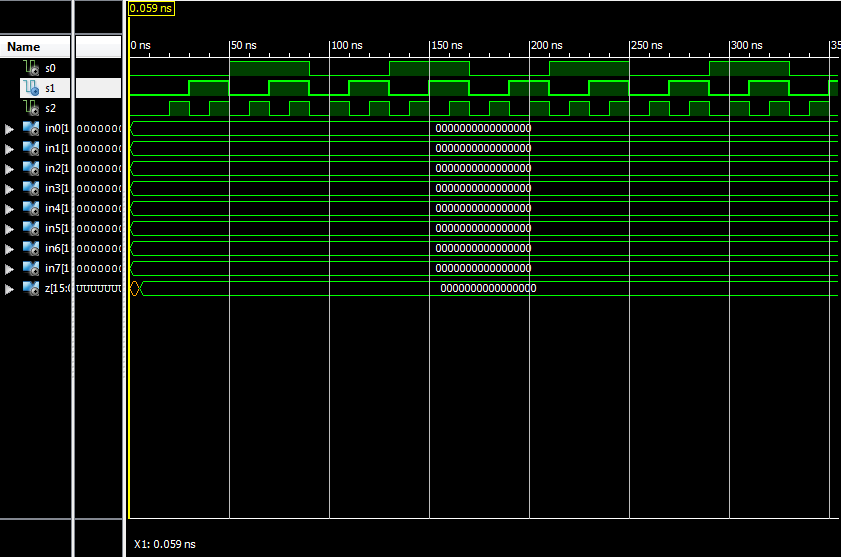
\includegraphics[width=16cm, height=8cm]{test_mux8.png}

	
\end{document}